\begin{chapter}{A path algebra SageMath class}
\label{appendix}
We have developed a \texttt{SageMath} class to deal with the long and tedious process of checking the hypotheses of the diamond lemma, and to automatically generate bases and compute some invariants of the Jacobian algebra associated to a polygonal subdivision, with the only input being the subdivision itself. We now present the source code, which we will then discuss in more detail:
\lstinputlisting{rewsystems.py}
We will explain how the program works by following an example execution in which we will compute some invariants of pyramids, as studied in \hyperref[pyramids]{Section \ref*{pyramids}}.

An instance of the \texttt{Rewriting\_System} class is constructed from an undirected graph representing a polygonal subdivison of the sphere. The associated quiver and standard potential will be automatically generated. We only implemented this feature for the spherical case since an enumeration of the faces of the polygonal subdivision is carried out by finding a planar embedding of the graph on the surface, and \texttt{SageMath} only provides such an algorithm for the sphere.

We would like to generate the rewriting system associated to a pyramid with an odd-sided base. In order to do that, we use the following snippet, which produces a pyramid with an $n$-sided base:
\begin{lstlisting}
def pyramid(n):
  edges = {}
  for i in xrange(1, n):
    edges[i] = [i+1, n+1]
  edges[n] = [1, n+1]
  return Graph(edges)
\end{lstlisting}
We now instantiate our desired triangulation:
\begin{lstlisting}
sage: odd_pyramid = pyramid(5)
sage: odd_pyramid.show()
\end{lstlisting}
\begin{figure}[h]
\centering
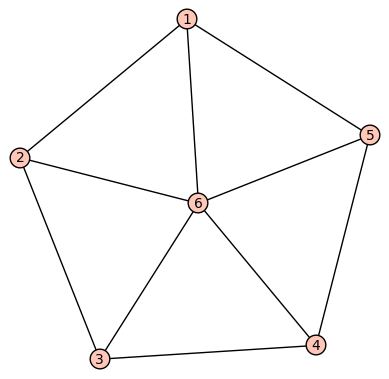
\includegraphics[width=0.5\textwidth]{odd_pyramid.png}
\end{figure}
Before producing the rewriting system, let us explain how the class constructor works. As mentioned previously, the QP will be automatically generated. If the \texttt{zero\_rules\_flag} is set to \texttt{False}, the \texttt{rewriting\_rules()} method will produce the set of usual rewriting rules (the ones associated to the grevlex order) and perform \hyperref[heuristic]{Heuristic \ref*{heuristic}} indefinitely until confluence is achieved. In order to test confluence, for every ambiguity we reduce both of its branches a maximum of \texttt{ambiguity\_depth} times and compare if both branches eventually resolve to the same element.

If the \texttt{zero\_rules\_flag} is set to \texttt{True}, the following heuristic will be executed just after producing the first set of rewriting rules, which are the ones that arise from the Jacobian relations:
\begin{heur} As we have seen in \hyperref[arbitrarily-long]{Observation \ref*{arbitrarily-long}},  any path that may be prolonged to a path of arbitrarily high length is zero. Reductions of the form $x\rightsquigarrow 0$ are highly desirable, since the ambiguities they generate are usually simple to resolve. Obviously, if $x=0$, then $yxz=0$ for all $y,z$, and so we are interested in finding only the shortest paths that reduce to zero. Therefore, we perform the following steps:
\begin{enumerate}
\item Let $n=2$.
\item Produce a list of all paths of length $n$.
\item Apply rewriting rules to each path until either they are irreducible or they are longer than \texttt{zero\_depth}.
\item If a path $x$ is equal to a path of length greater than \texttt{zero\_depth}, add the rewriting rule $x\rightsquigarrow 0$.
\item If no path was found to reduce to zero, increase $n$ by 1 and repeat steps 2 to 5.
\end{enumerate}
This may be formalized by a \textcolor{red}{pumping lemma argument} if we choose a high enough value for \texttt{zero\_depth}.
\end{heur}

We now generate the rewriting system associated to our pyramid:
\begin{lstlisting}
sage: odd_rs = Rewriting_System(odd_pyramid)
9 rules added.
4 rules added.
Total rules: 33
\end{lstlisting}
As we can see, the program had to enlarge the set of rules twice before achieving confluence. Let us examine the quiver and its associated potential, which both were generated automatically out of the triangulation:
\begin{lstlisting}
sage: odd_rs.quiver.show()
\end{lstlisting}
\begin{figure}[h]
\centering
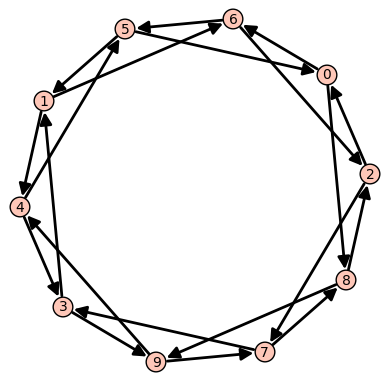
\includegraphics[width=0.5\textwidth]{odd_quiver.png}
\end{figure}
\begin{lstlisting}
sage: odd_rs.potential
[[8, 5, 6, 8],
 [3, 4, 6, 3],
 [0, 3, 5, 7, 1, 0],
 [7, 8, 9, 7],
 [1, 9, 2, 1],
 [4, 0, 2, 4],
 [0, 2, 1, 0],
 [0, 3, 4, 0],
 [3, 5, 6, 3],
 [5, 7, 8, 5],
 [1, 9, 7, 1],
 [2, 4, 6, 8, 9, 2]]
\end{lstlisting}
As the output shows, there are five 3-cycles coming from the triangular faces, a 5-cycle from the pentagonal face, five 3-cycles from punctures where three faces meet and another 5-cycle from the puncture corresponding to the apex of the pyramid.

The confluent rewriting system found by the software is given by this set of 33 rules:
\begin{lstlisting}
sage: odd_rs.rules
{(0, 2, 1): -(0, 3, 5, 7, 1),
 (0, 2, 4): -(0, 3, 4),
 (1, 0, 2): -(1, 9, 2),
 (1, 0, 3, 4): (1, 9, 2, 4),
 (1, 0, 3, 5, 6): -(1, 9, 2, 4, 6),
 (1, 0, 3, 5, 7, 8): (1, 9, 2, 4, 6, 8),
 (1, 9, 2, 4, 6, 8, 9, 7): (1, 0, 3, 5, 7, 1, 0, 3, 5, 7),
 (1, 9, 7): -(1, 0, 3, 5, 7),
 (2, 1, 0): -(2, 4, 0),
 (2, 1, 9): -(2, 4, 6, 8, 9),
 (3, 4, 0): -(3, 5, 7, 1, 0),
 (3, 4, 6): -(3, 5, 6),
 (4, 0, 2): -(4, 6, 8, 9, 2),
 (4, 0, 3): -(4, 6, 3),
 (5, 6, 3): -(5, 7, 1, 0, 3),
 (5, 6, 8): -(5, 7, 8),
 (5, 7, 1, 0, 3, 4): -(5, 7, 8, 9, 2, 4),
 (6, 3, 4): -(6, 8, 9, 2, 4),
 (6, 3, 5): -(6, 8, 5),
 (6, 8, 9, 2, 4, 0): (6, 8, 9, 7, 1, 0),
 (7, 1, 0, 3, 5, 6): (7, 8, 9, 2, 4, 6),
 (7, 1, 9): -(7, 8, 9),
 (7, 8, 5): -(7, 1, 0, 3, 5),
 (7, 8, 9, 7): (7, 1, 0, 3, 5, 7),
 (8, 5, 6): -(8, 9, 2, 4, 6),
 (8, 5, 7): -(8, 9, 7),
 (8, 9, 2, 4, 6, 3): -(8, 9, 7, 1, 0, 3),
 (9, 2, 1): -(9, 7, 1),
 (9, 2, 4, 0): (9, 7, 1, 0),
 (9, 2, 4, 6, 3): -(9, 7, 1, 0, 3),
 (9, 2, 4, 6, 8, 5): (9, 7, 1, 0, 3, 5),
 (9, 2, 4, 6, 8, 9, 7): -(9, 7, 1, 0, 3, 5, 7),
 (9, 7, 8): -(9, 2, 4, 6, 8)}
\end{lstlisting}
Rules are stored as a dictionary, where keys are reducible monomials. The value associated to a key is a \texttt{Term} object, which consists of a monomial and a sign, representing the term into which the key reduces.

We may now compute the set of all irreducible paths up to a certain length. This is performed by just filtering the list of all paths. For instance, we may produce the list of all irreducible paths of length 4:
\begin{lstlisting}
sage: odd_rs.basis(5)[-1]
[[0, 3, 5, 7, 1],
 [0, 3, 5, 7, 8],
 [1, 0, 3, 5, 7],
 [1, 9, 2, 4, 6],
 [2, 4, 6, 8, 5],
 [2, 4, 6, 8, 9],
 [3, 5, 7, 1, 0],
 [3, 5, 7, 8, 9],
 [4, 6, 8, 9, 2],
 [4, 6, 8, 9, 7],
 [5, 7, 1, 0, 3],
 [5, 7, 8, 9, 2],
 [6, 8, 9, 2, 4],
 [6, 8, 9, 7, 1],
 [7, 1, 0, 3, 5],
 [7, 8, 9, 2, 4],
 [8, 9, 2, 4, 6],
 [8, 9, 7, 1, 0],
 [9, 2, 4, 6, 8],
 [9, 7, 1, 0, 3]]
\end{lstlisting}
The \texttt{irred\_paths()} method counts the number of irreducible paths up to a specified length:
\begin{lstlisting}
sage: odd_rs.irred_paths(15)
[10, 20, 20, 20, 20, 20, 20, 20, 20, 20, 20, 20, 20, 20, 20]
\end{lstlisting}

Finally, we include a snippet that generate the triangulations corresponding to prisms and antiprisms:

\begin{lstlisting}
def prism(n):
    edges = {}
    for i in xrange(1, n):
        edges[i] = [i+1, i+n]
        edges[i+n] = [i+n+1]
    edges[n] = [1, 2*n]
    edges[2*n] = [n+1]
    return Graph(edges)

def antiprism(n):
    edges = {}
    for i in xrange(1, n):
        edges[i] = [i+1, i+n]
        edges[i+n] = [i+n+1, i+1]
    edges[n] = [1, 2*n]
    edges[2*n] = [1, n+1]
    return Graph(edges)
\end{lstlisting}
\end{chapter}